\begin{frame}[t]{Aplicação: transporte de peças na indústria}
\begin{columns}[T,onlytextwidth]
\begin{column}{0.62\textwidth}
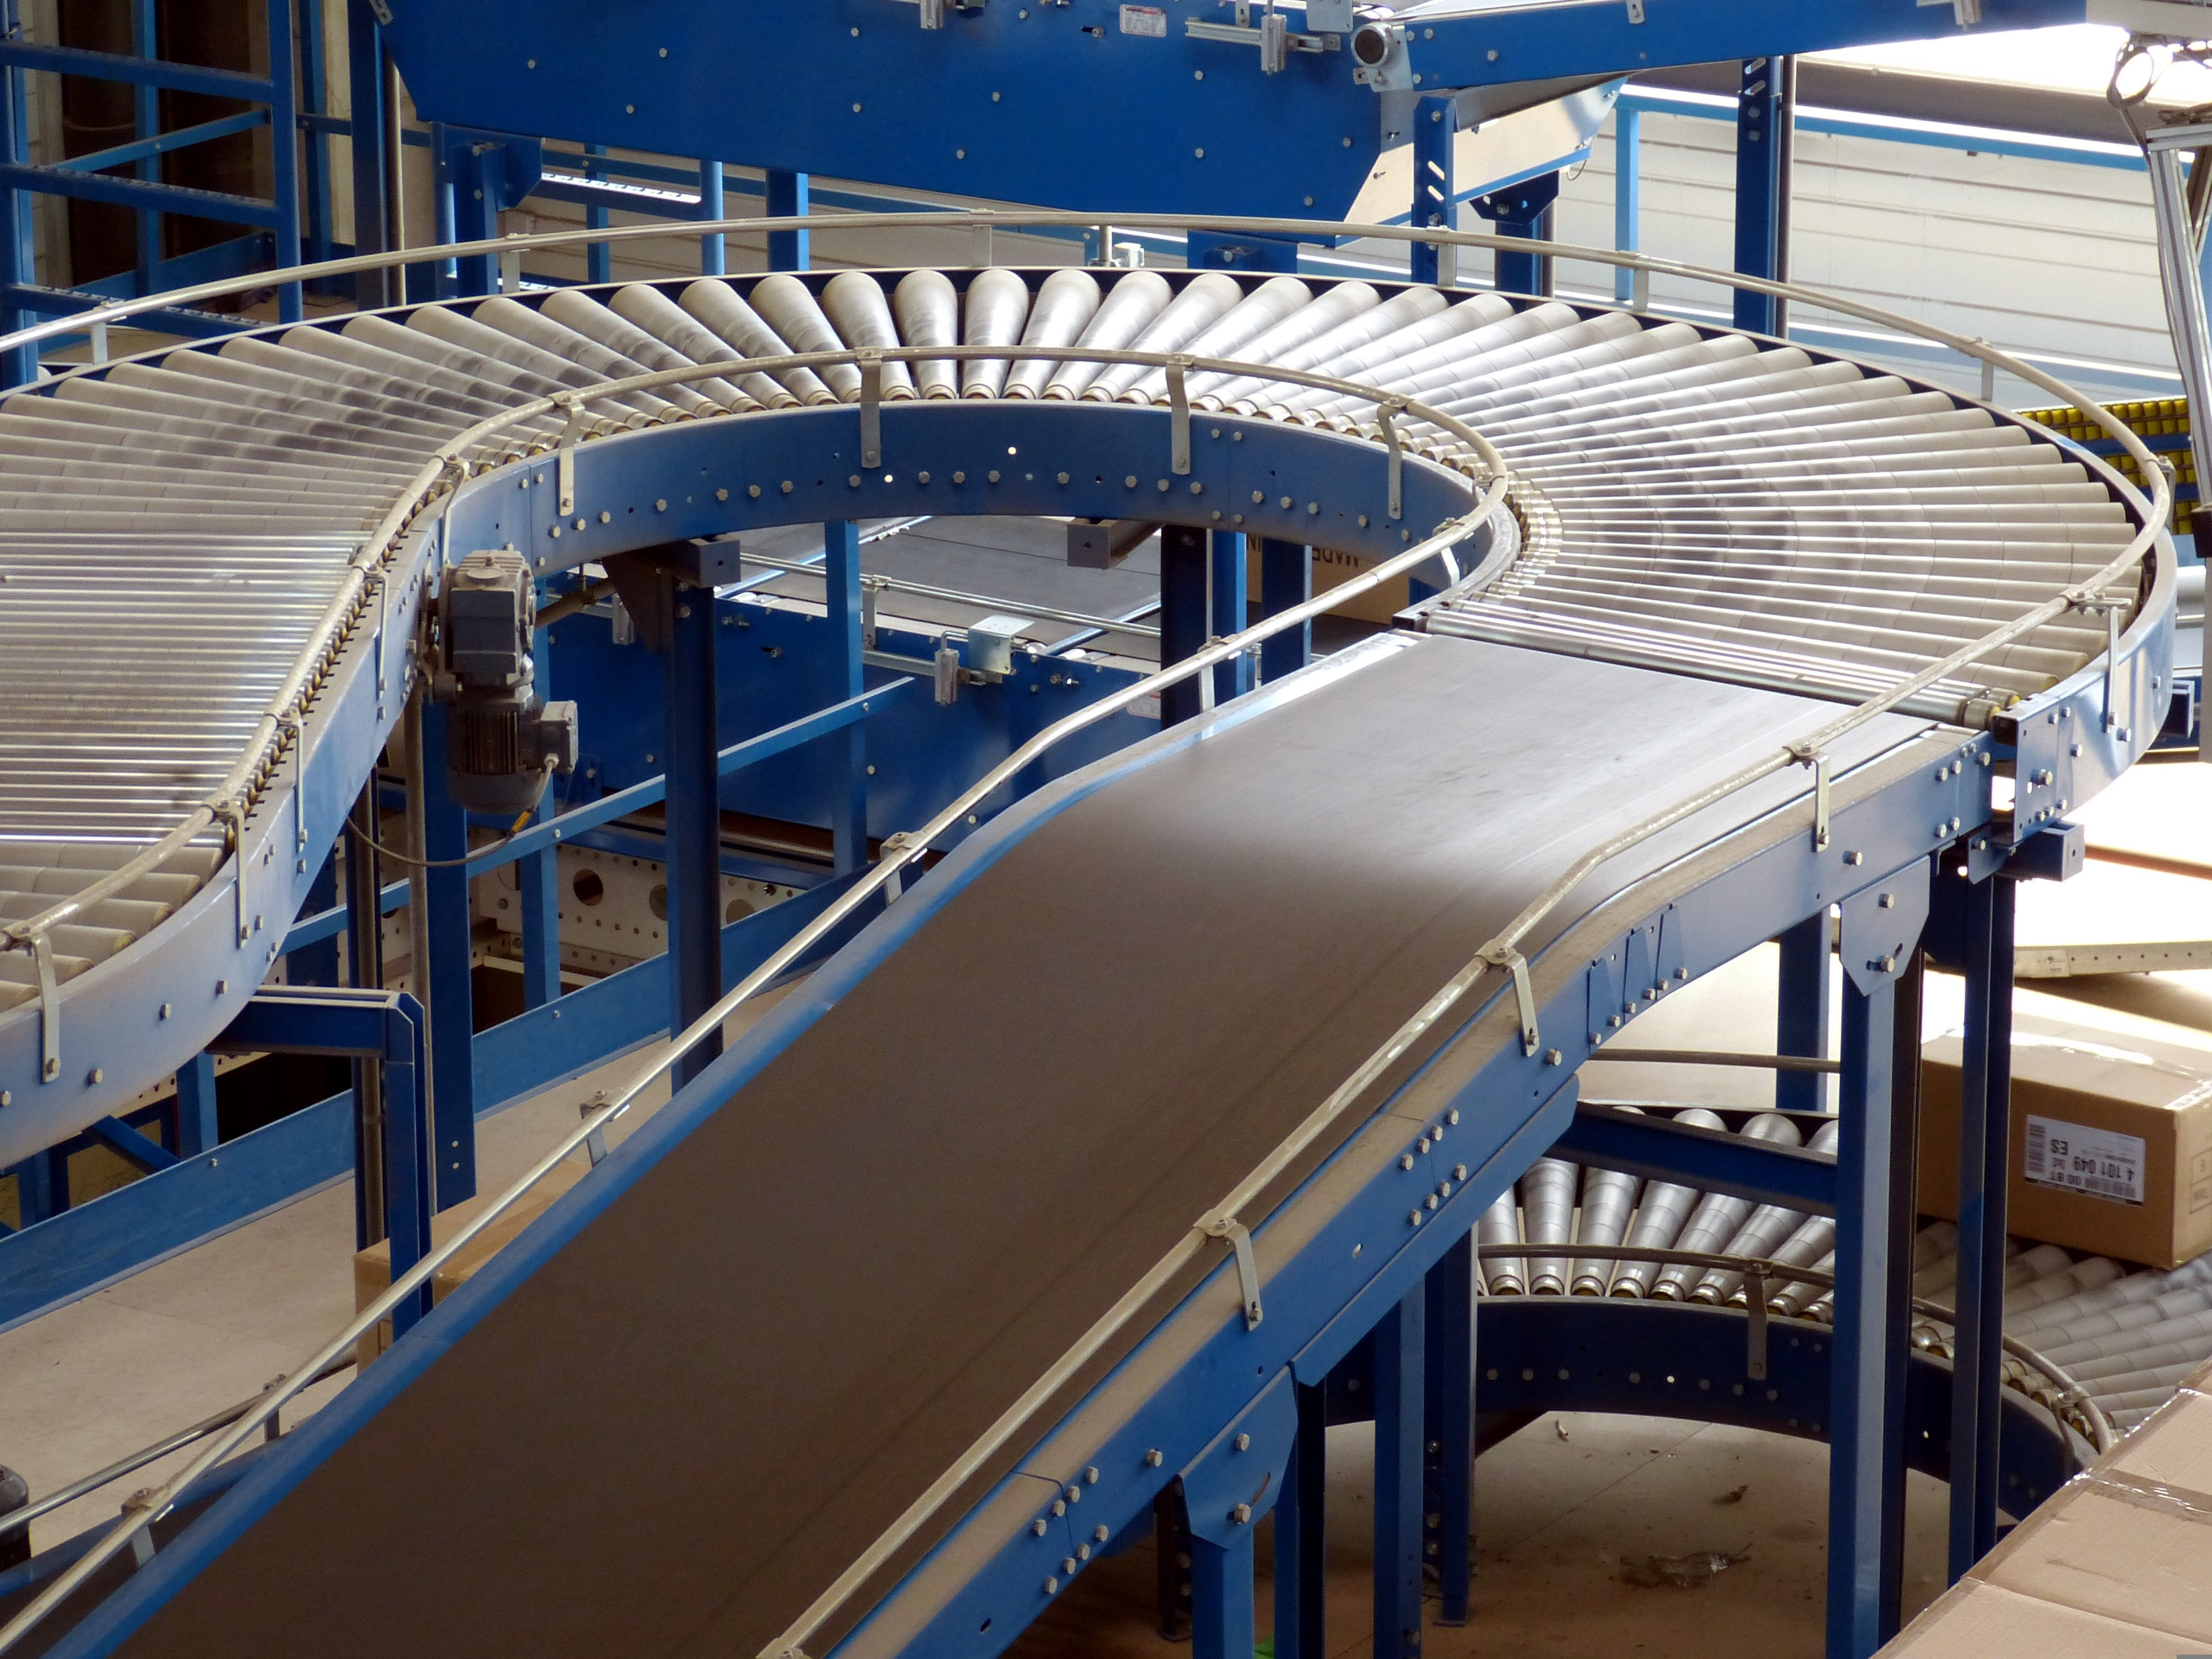
\includegraphics[width=\linewidth,height=4.7cm,keepaspectratio]{images/esteira_industrial.jpg}
\end{column}
\begin{column}{0.35\textwidth}
\small
\textbf{Relação com o modelo}
\begin{itemize}
\item Iniciar: solicita o movimento.
\item Motor: aciona o transporte.
\item Sensor: indica a chegada da peça.
\item Pronto: sinaliza o fim do ciclo.
\end{itemize}
\end{column}
\end{columns}
\medskip
\footnotesize A foto contextualiza o transporte industrial. A máquina de estados apresentada é um modelo didático simplificado.
\end{frame}
